\section{Nutrient Groups}\label{sec:nutrient_group}

\subsection{View Nutrient Group List}\label{sec:nutrient_group_list}
\setcounter{stepcounter}{1}
\paragraph{\arabic{stepcounter}.}Expand \textcolor{ForestGreen}{"Group"} menu and click on \textcolor{ForestGreen}{"Nutrient Group"}
\begin{figure}[h!]
  	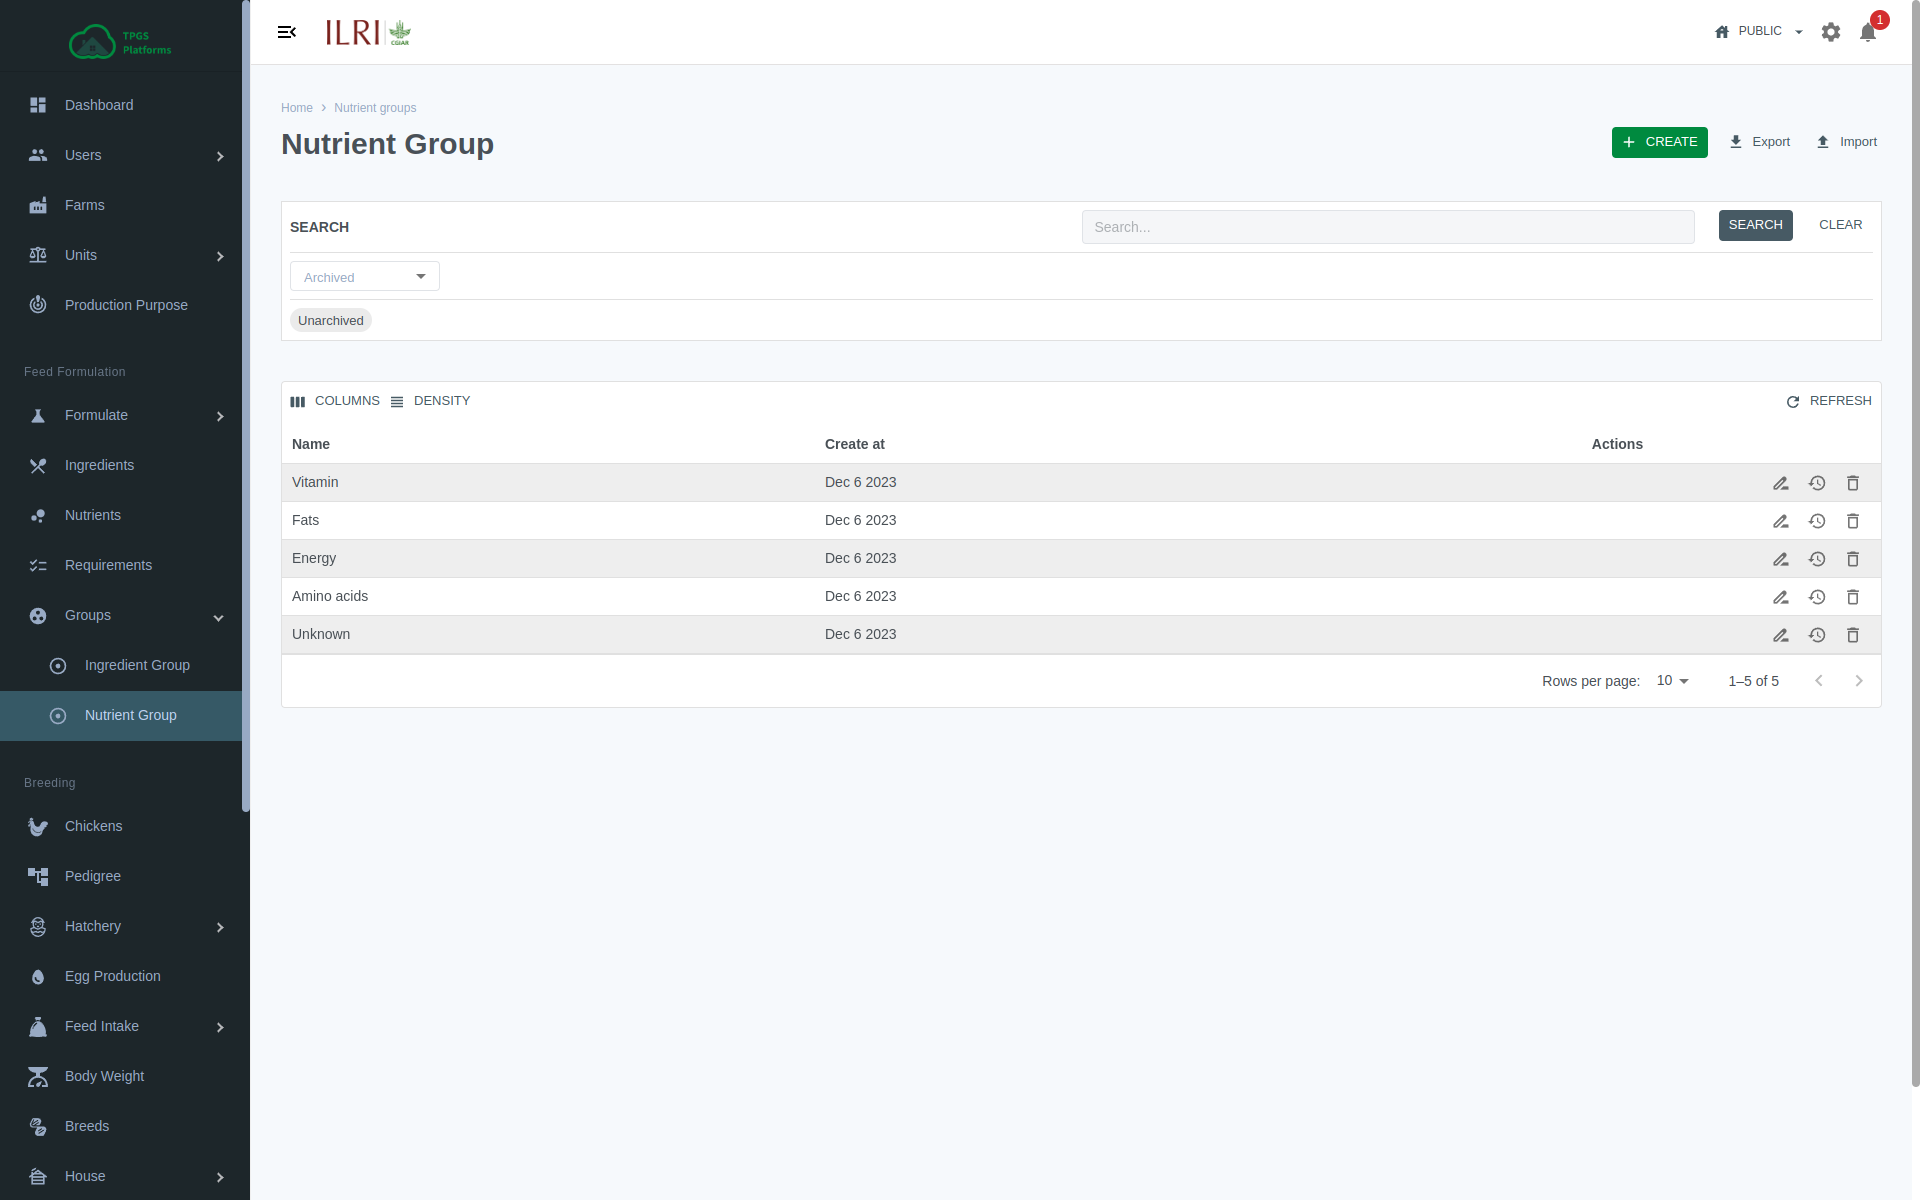
\includegraphics[width=15cm]{screenshots/nutrient_group_list_page.png}
  	\caption{Nutrient Group List}
  	\label{fig:nutrient_group_list_page}
\end{figure}

\subsection{Archive Records}\label{sec:nutrient_group_list_archived}
\setcounter{stepcounter}{1}
\paragraph{\arabic{stepcounter}.}On filter section filter the records by archive.

\subsection{Create new Nutrient Group}\label{sec:nutrient_group_create}
\setcounter{stepcounter}{1}
\paragraph{\arabic{stepcounter}.}To create new nutrient group click on \textcolor{ForestGreen}{"Create"} \hyperref[fig:nutrient_group_list_page]{Refer from nutrient list Figure \ref{fig:nutrient_group_list_page}}
\begin{figure}[h!]
  	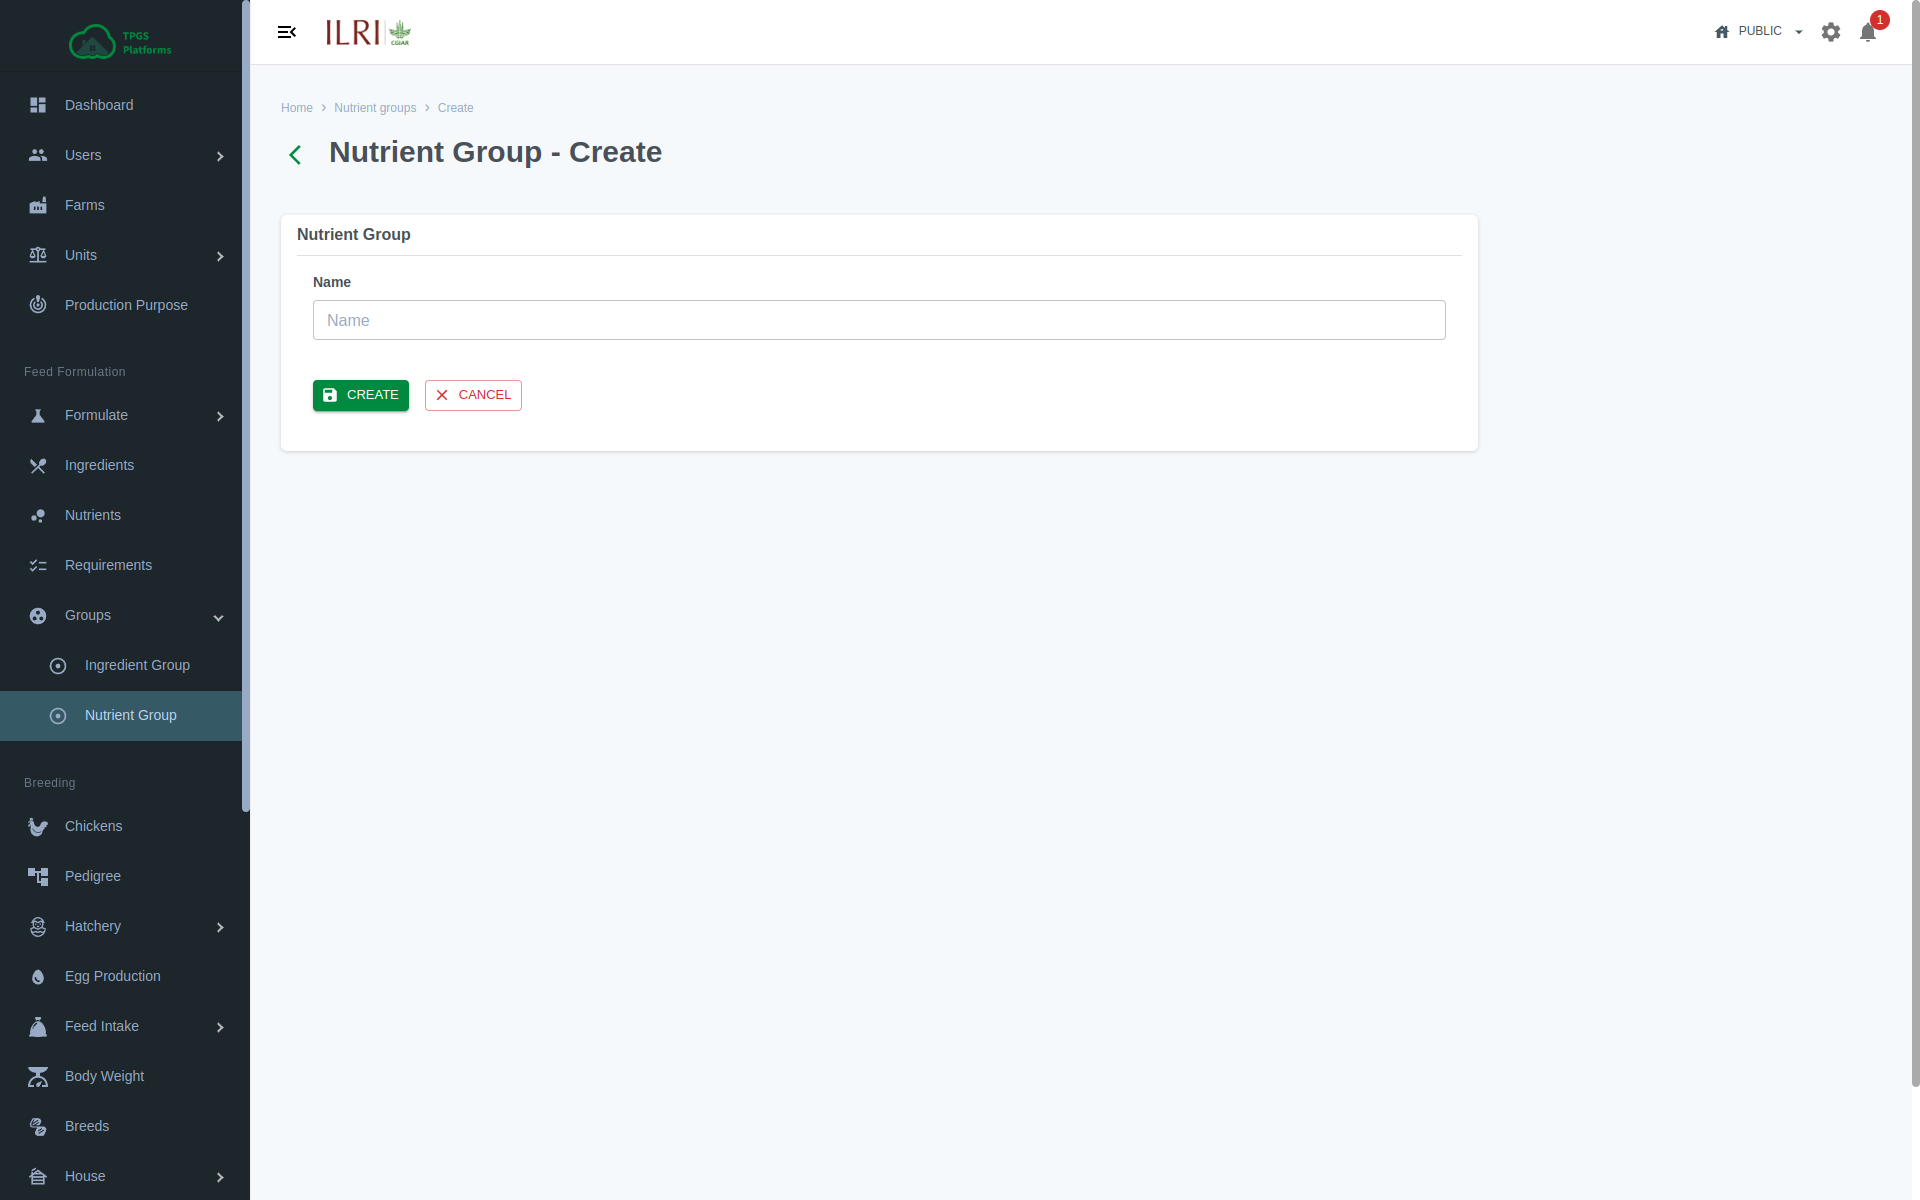
\includegraphics[width=15cm]{screenshots/nutrient_group_create_page.png}
  	\caption{Create new Nutrient Group}
  	\label{fig:nutrient_group_create_page}
\end{figure}
And click \textcolor{ForestGreen}{"CREATE"}, you will be redirect to  \hyperref[sec:nutrient_group_list]{Nutrient List section \ref{sec:nutrient_group_list}}

\subsection{Edit Nutrient Group}\label{sec:nutrient_group_edit}
\setcounter{stepcounter}{1}
\paragraph{\arabic{stepcounter}.}Go to the Nutrient Group \hyperref[sec:nutrient_group_list]{Refer to Section \ref{sec:nutrient_group_list}}, then click on Pencil icon and it will redirect to the \hyperref[fig:nutrient_group_edit_page]{Figure \ref{fig:nutrient_group_edit_page}}.
\begin{figure}[h!]
  	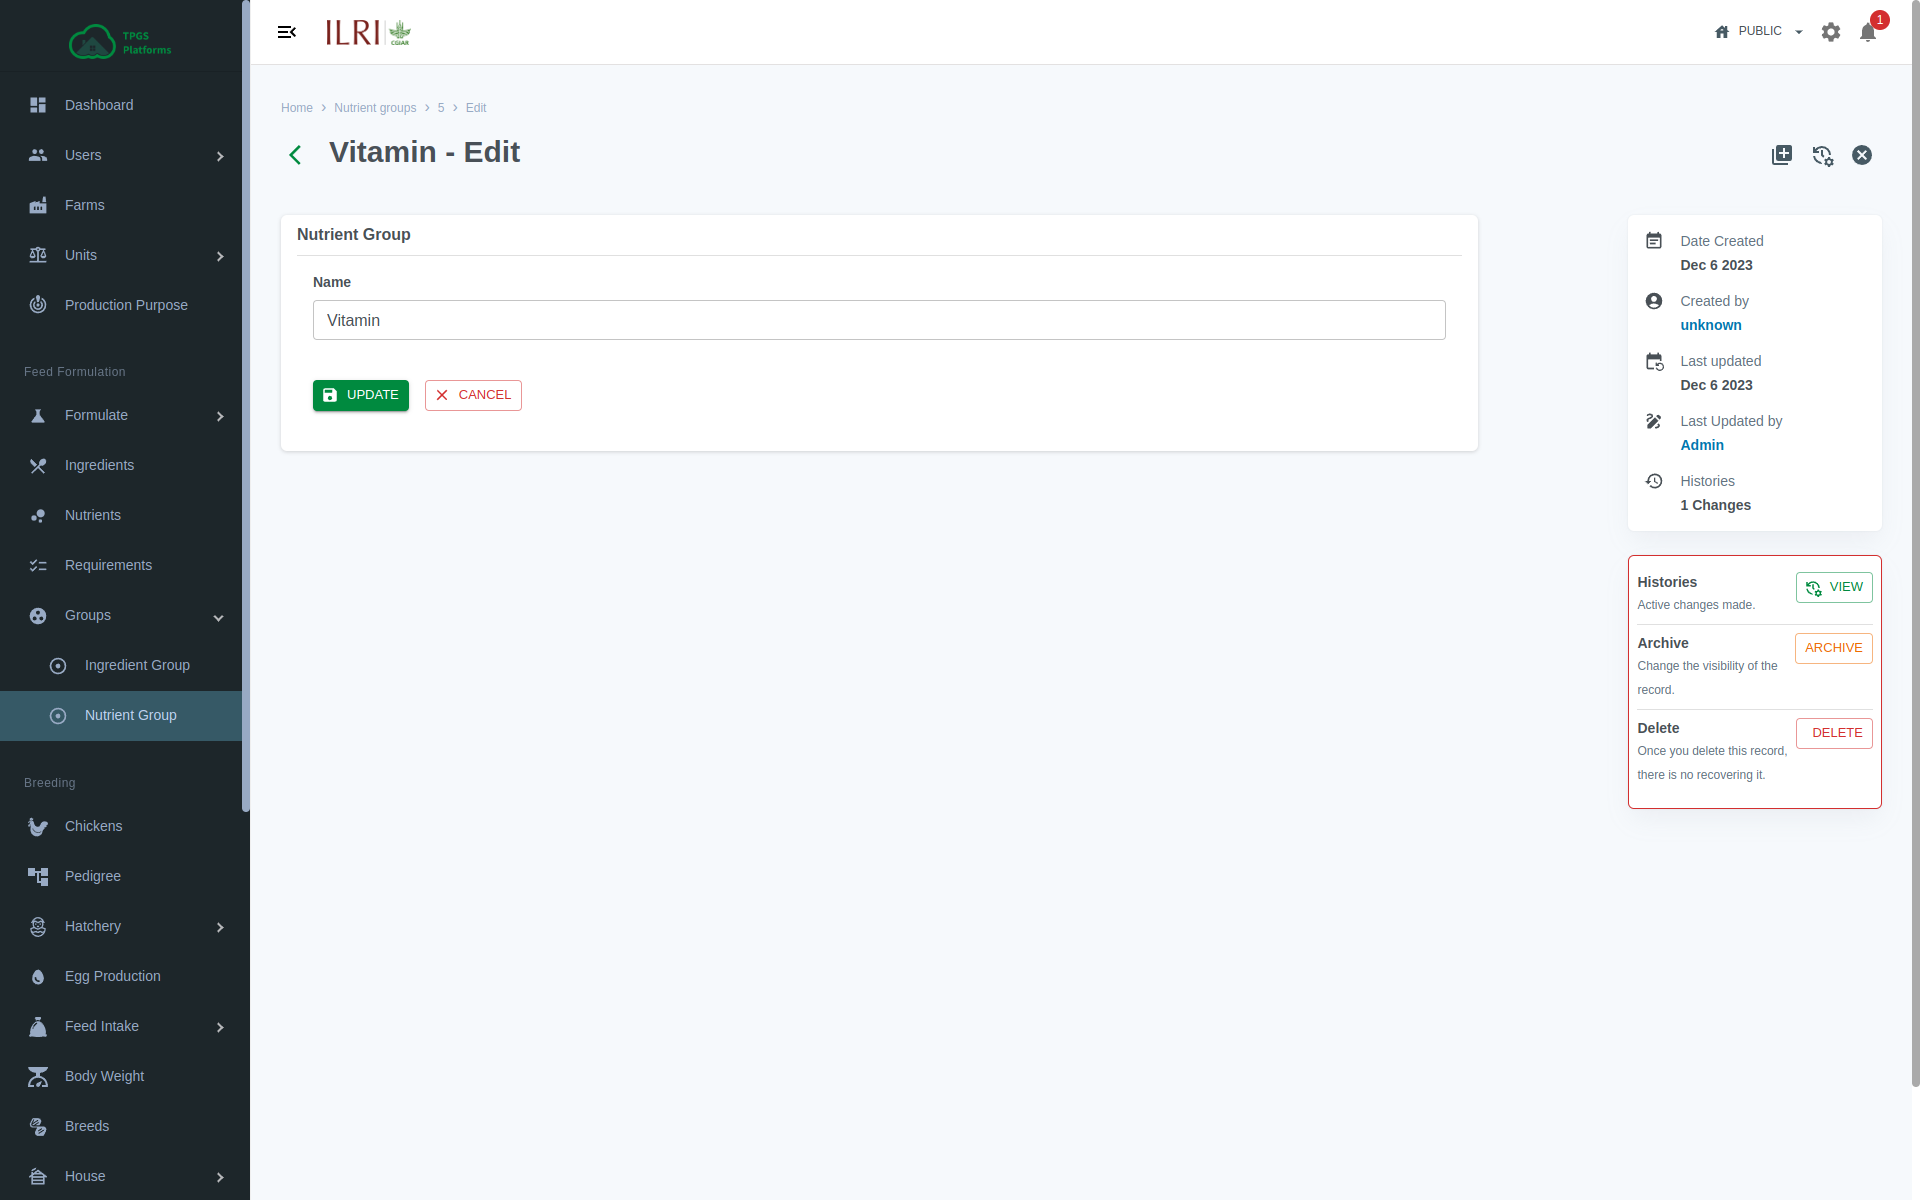
\includegraphics[width=15cm]{screenshots/nutrient_group_edit_page.png}
  	\caption{Edit Nutrient Group}
  	\label{fig:nutrient_group_edit_page}
\end{figure}

\subsection{Delete Nutrient Group}
\setcounter{stepcounter}{1}
\paragraph{\arabic{stepcounter}.}Go to the edit Nutrient Group \hyperref[sec:nutrient_group_edit]{Refer to Section \ref{sec:nutrient_group_edit}}.

\paragraph{\arabic{stepcounter}.}To archive the record click on \textcolor{ForestGreen}{"Archive"}. If you want to bring back the record/unarchive follow the step under \hyperref[sec:nutrient_group_list_archived]{Section  \ref{sec:nutrient_group_list_archived}}, and click on \textcolor{ForestGreen}{"UnArchive"}


\paragraph{\arabic{stepcounter}.}To permanently delete the record click on \textcolor{ForestGreen}{"Delete"}.

\begin{figure}[h!]
  	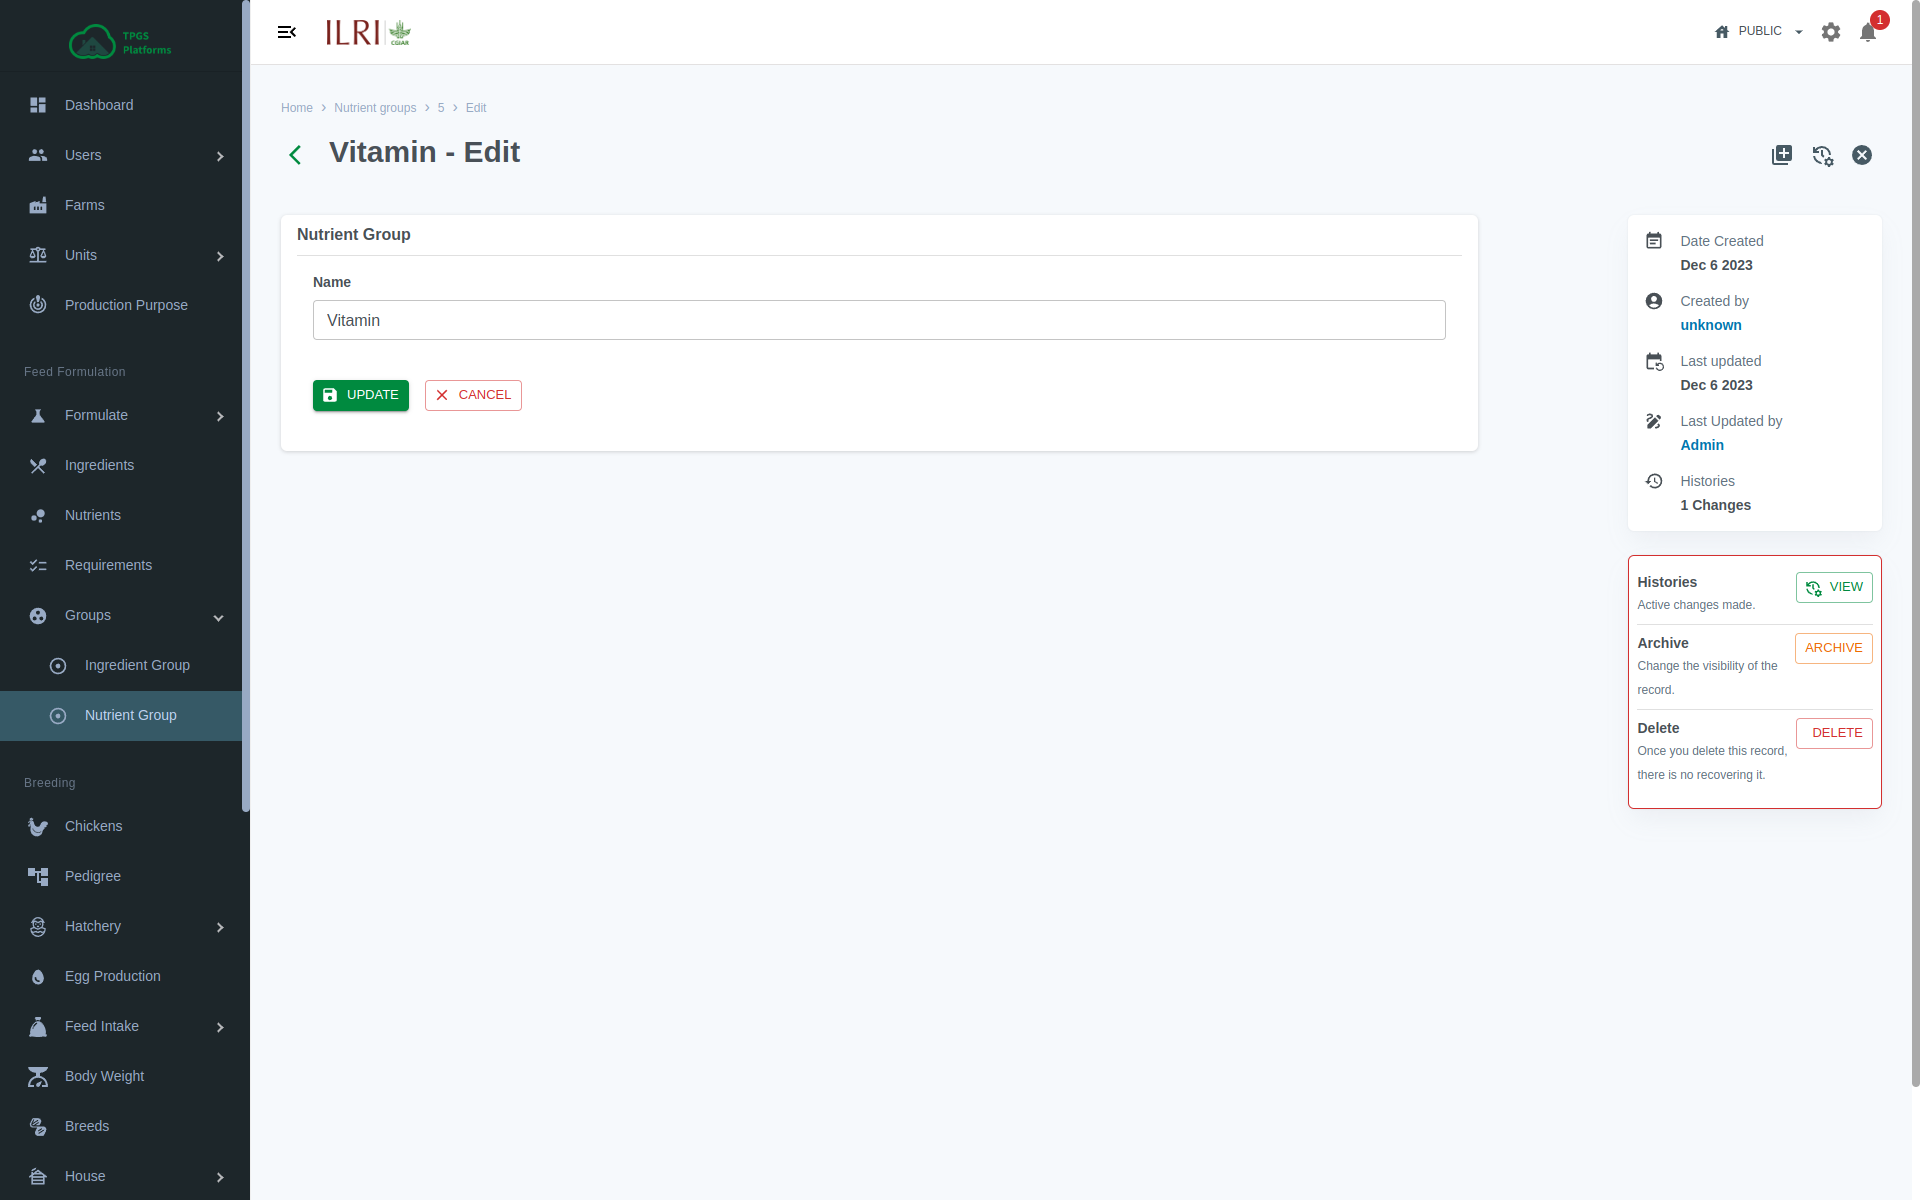
\includegraphics[width=15cm]{screenshots/nutrient_group_edit_page.png}
  	\caption{Edit Nutrient Group}
  	\label{fig:nutrient_group_edit_page}
\end{figure}